\section{Distributed Model Checking} \label{sec::DMC}
In addition to benefiting from the isolation of actors for reducing the size of state spaces, this property can be used for more efficient analysis of huge state spaces. A major limiting factor in applying model checking for the analysis of real-world systems is the huge amount of space and time required to store and explore state spaces. Distributed model checking is a technique for analyzing the state space in which state space is partitioned into slices and each slice is assigned to a computational node to be analyzed. Efficiency of this technique depends on the communication cost among the computational nodes which is related to the distribution policy of states among the nodes \cite{DBLP:journals/entcs/OrzanPE05}.
%
%Another, more fine-grained, representative of communication cost 
An specific measurement for communication cost is the number of split transitions; a split transition is a transition between two states  where the hosts of source and destination states are different nodes. In \cite{DBLP:journals/eceasst/KhamespanahSMSR15} we show how the actor model can be used to reduce the number of split transitions. We introduce a new state distribution policy based on the so-called \textit{Call Dependency Graph (CDG)} of actor models. A CDG represents the abstract causality relation among messages of actors. Our abstraction is akin to the Clinger's event Diagram \cite{clinger} that is a dynamic representation of actor's event activation causality. 
\fixme{what do you mean by dynamic representation?}
%dynamic representation of actor's event activation causality proposed by Clinger \cite{clinger}. 

The most primitive and widely used distribution policy is random state distribution \cite{DBLP:journals/entcs/GaravelMS13}. Random state distribution policy distributes states among nodes based on their hash values. Random distribution policy guarantees load balancing. However, it is not an effective technique as cycles are scattered over many different nodes. In \cite{DBLP:journals/entcs/OrzanPE05}, another state space distribution policy is suggested to improve the locality of cycles. \fixme{in one sentence define locality here} This policy is based on the static analysis of an abstracted model and detects \emph{may} or \emph{must} transition relations among states \cite{DBLP:conf/lics/LarsenT88}.
\fixme{define may and must in one sentence}
Based on this analysis, if two states have a \emph{must} relation, they should be stored in a same node. We use a similar idea in our state distribution policy and show that using the CDG improves the locality of cycles by reducing the split transitions in the state space. In other words, we find the \emph{must} relations among the states of actor models using the CDG. Our technique is applicable to other service-oriented
\fixme{why you are talking about service-oriented here? maybe reactive distributed systems?}
models where the unit of concurrency can be modeled as isolated autonomous reactive objects and message passing is the only way of communication. 

Clinger's event diagram comprises vertices (called \emph{dots}) for each event, and edges (called \emph{arrows}) that represent the activation relation of two events. Clinger's event diagram is typically drawn using parallel vertical swim-lanes for each actor, where the dots are placed for each event respecting their sequential execution order. Figure~\ref{fig::clinger} represents the Clingers' event diagram of a simple actor model, shown in Listing~\ref{src::actor-model}. 

\begin{lstlisting}[language=rebeca, caption= A simple actor model, label=src::actor-model]
reactiveclass AC1 {
   knownrebecs {AC2 ac2;}
   AC1() {
     self.msg1();
   }
   msgsrv msg1() {
     self.msg2();
     ac2.msg3();
   }
   msgsrv msg2() {
     self.msg1();
     ac2.msg4();
   }
}
reactiveclass AC2 {
   knownrebecs{AC1 ac1;}
   statevars{int sv;}
   AC2() {
     sv = 1;
   }
   msgsrv msg3() {
     ac1.msg1();
   }
   msgsrv msg4() {
     if (sv == 1)
       sv = 4;
     else
       sv = 3;
   }
}
main {
    AC1 ac1(ac2):();
    AC2 ac2(ac1):();
}
\end{lstlisting}

Clinger's event diagrams can be seen as the detailed representations of CDG. Intuitively, a CDG represents the possible activation relations of events derived from a static analysis of the model. Note that as actors are isolated, the only mechanism which may result in activating an event (causality among events) in an actor is sending a message to it. So, the activation relation of events in a CDG can be extracted from the %source code of the 
actor model by analyzing the message passing among actors. Using static analysis to find message passing, results in an over-approximation of events activations in CDGs. Figure \ref{fig::cdg} illustrates the CDG which corresponds to the Clinder's event diagram of Figure \ref{fig::clinger}.

\begin{figure}
\centering
\subfigure[Clinger event diagram of the actor model in Listing 1]{
\label{fig::clinger}
  \centering
  \small{
   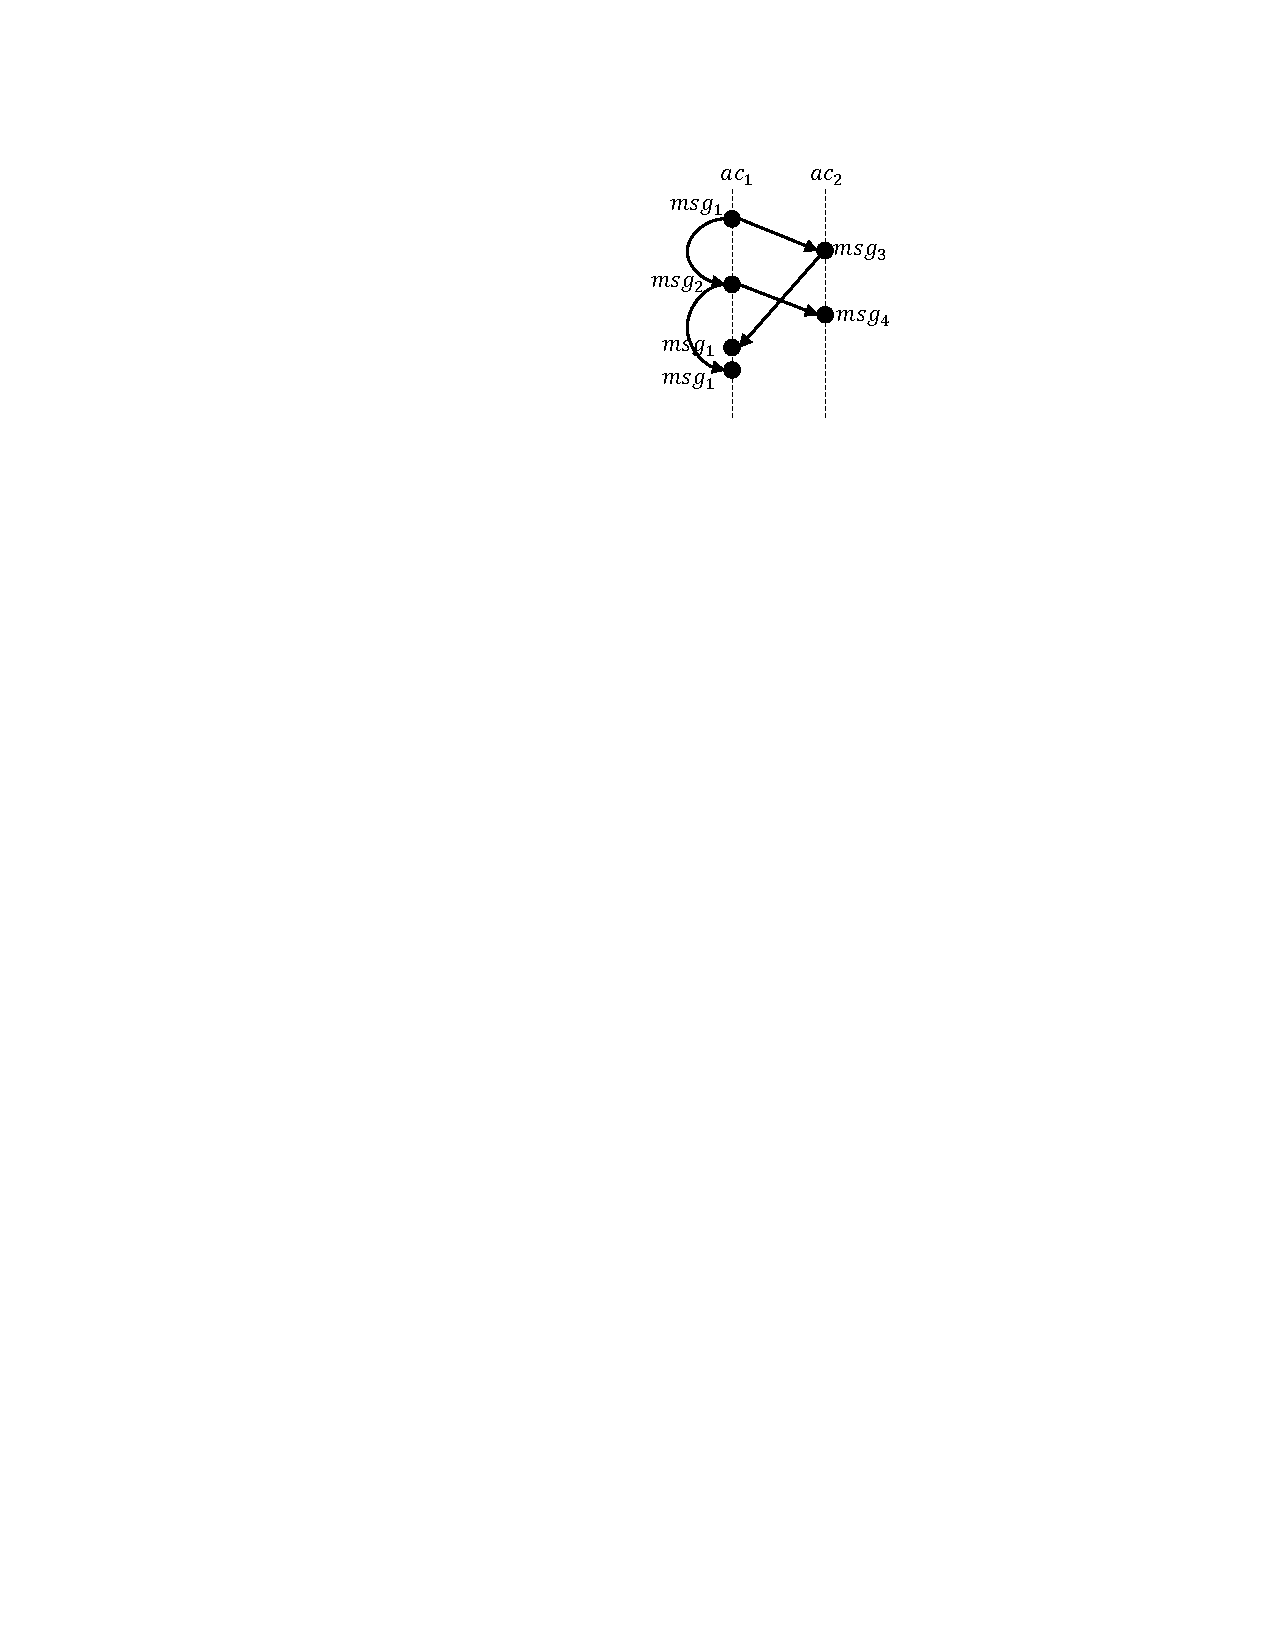
\includegraphics[width=.18\textwidth]{resources/clinger.pdf}
  }
}
\qquad
\subfigure[CDG of the actor model in Listing 1]{
\label{fig::cdg}
  \centering
  \small{
   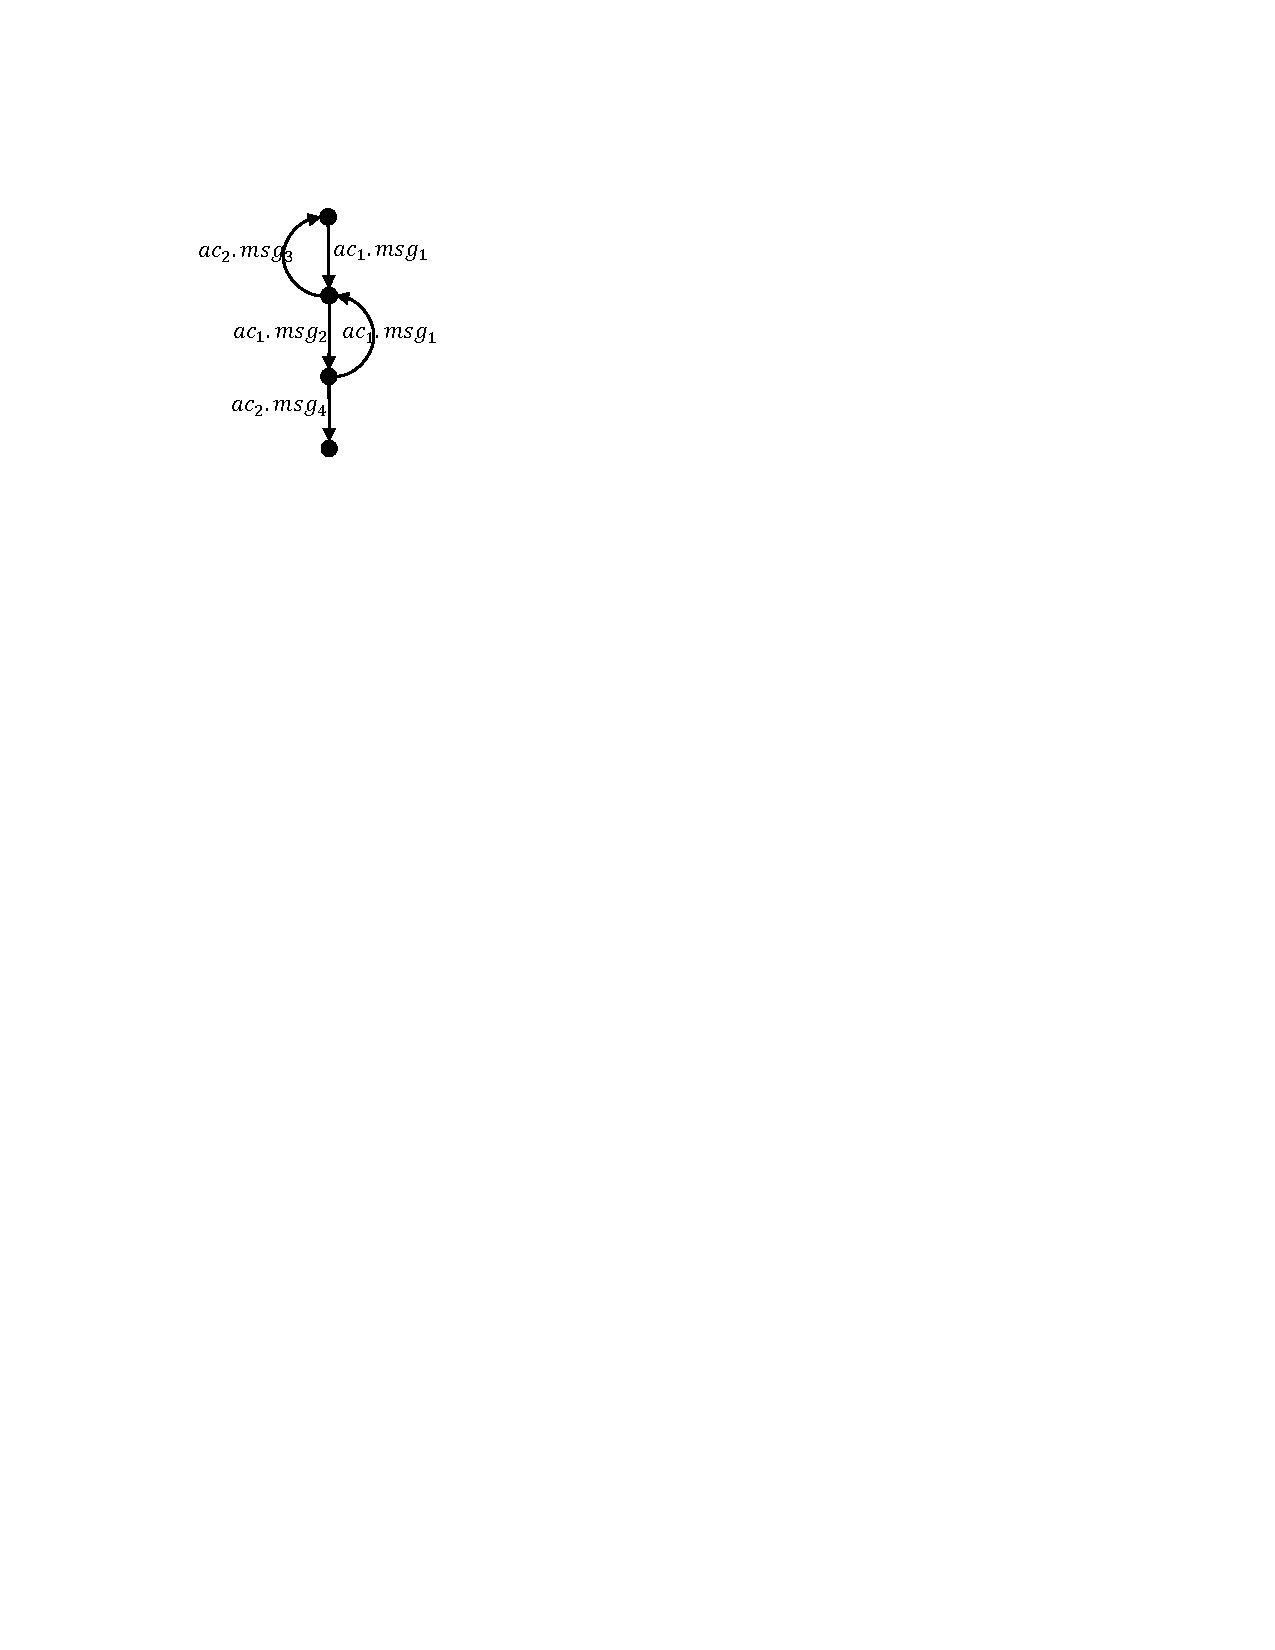
\includegraphics[width=.18\textwidth]{resources/cdg.pdf}
  }
}
\caption{Clinger event diagram versus CDG of the actor model in Listing 1.}
\label{fig::clinger-cdg}
\end{figure}

In \cite{DBLP:journals/eceasst/KhamespanahSMSR15} we designated and proved a relation between the cycles in the CDG and the cycles in the state space. We devised a distribution policy for the distributed model checker of \emph{Rebeca} based on the CDG. The new distribution policy increases the efficiency of distributed model checking by increasing the locality of the accepting cycles.
\fixme{you are talking about locality of the accepting cycles and cycles, you are not explaining the differences, which one is more important? }
\fixme{You are not saying why isolation helps here, why other cannot find such relation?}
Experimental evidence supports that this new policy improves cycle locality, and decreases model checking time and memory in practice.